\chapter{Portierung des Laufplaners nach ROS und Gazebo}

\section{Analyse bestehender Laufplaner}

Herms, Ruffler + ---> verlinken: Die Darstellung geschieht mit Hilfe der 3D- Bibliothek OpenInventor [33]

\section{Vorgehensweise und Aufbau des Pakets}

Die zuvor analysierten Laufplaner müssen nun in das \ac{ROS} portiert werden. Ferner muss der Algorithmus zur Laufplanung extrahiert und mit \ac{ROS} kompatibel gemacht werden. Dabei gibt es einige Herausforderungen, die gelöst werden müssen:
\begin{itemize}
  \item Code-technisch ist der Laufplaner \textit{fest verdrahtet mit dem Terrain der OpenInventor-Oberfläche}, während das neue Paket auf Gazebo laufen soll.
  \item Der Laufplaner nutzt für geometrische Berechnungen \textit{Klassen aus der OpenInventor-Bibliothek}, während \ac{ROS} auf die Klassen des TF-Frameworks zurückzugreifen soll.
  \item Durch \textit{unterschiedliche Robotermodelle} können Maße innerhalb des Codes anders definiert sein und müssen angepasst werden.
\end{itemize}

Da eine komplette Kopie des vorherigen Projekts auf Grund verschiedener Umgebungen nicht möglich ist, ist die Vorgehensweise schrittweise wichtige Codestellen zu übertragen und zu testen. Dies hat den Vorteil, dass Funktionen unabhängig voneinander getestet werden können. Damit ergibt sich der folgende Gesamtablauf für die Portierung:
\begin{enumerate}
  \item Aufsetzen des \ac{ROS}-Pakets
  \item Aufsetzen der Simulation
  \begin{enumerate}
    \item Aufsetzen des Roboter-Modells
    \item Aufsetzen der Gelenkmotoren
  \end{enumerate}
  \item Aufsetzen der Fußsteuerung
  \item Testen der Fußsteuerung
  \item Portierung des Laufalgorithmus
\end{enumerate}

Während der Arbeit hat es sich als sinnvoll herausgestellt, die Portierung erst zum Schluss zu beginnen. Der Grund dafür ist, dass es damit während der Portierung möglich ist schon Artefakte in der Simulation zu testen. Damit lässt sich wesentlich besser einschätzen, ob das Übertragene auch funktioniert. Außerdem basiert der Laufplaner auf Funktionalitäten wie dem Roboter-Modell und der Definition der Gelenkmotoren. Mit dieser Vorgehensweise kann das Paket nun schrittweise implementiert werden.

\autoref{Kap4:ROSPackageFolderStructure} definiert die Ordnerstruktur des \ac{ROS}-Pakets. Die Ordnerstruktur ist typisch für \ac{ROS}-Pakete und findet sich ähnlich in vielen weiteren Paketen der \ac{ROS}-Community. Der Aufbau des Pakets ist an das Akrobat-Paket \autocite{akrobat} sowie das Hopper-Paket \autocite{hopper} angelehnt. Beide Pakete nutzen wichtige Konzepte für das Robotermodelle und die Gelenksteuerung, die auch für dieses Projekt wichtig sind.

\begin{figure}[p!]
\dirtree{%
.1 hexapod.
.2 config.
.3 config.rviz.
.3 hexapod.yaml.
.2 urdf.
.3 hexapod.xacro.
.3 leg-1.xacro.
.3 leg-2.xacro.
.3 leg-3.xacro.
.3 leg-4.xacro.
.3 leg-5.xacro.
.3 leg-6.xacro.
.2 launch.
.3 rviz.launch.
.3 gazebo.launch.
.3 model.launch.
.3 akrobat\_walk.launch.
.3 control.launch.
.2 include.
.3 akrobat.
.4 akrobat\_init.h.
.4 JointStateToGazebo.h.
.4 ControlRandomSampling.h.
.4 JointStateToDynamixel.h.
.4 FootConfiguration.h.
.4 Akrobat.h.
.3 pugixml.
.2 worlds.
.3 default.world.
.2 stl.
.3 hexapod\_link.stl.
.3 coxa\_r\_link.stl.
.3 coxa\_l\_link.stl.
.3 femur\_link.stl.
.3 tibia\_link.stl.
.2 src.
.3 akrobat.
.4 akrobat\_main.cpp.
.4 JointStateToGazebo.cpp.
.4 FootConfiguration.cpp.
.4 JointStateToDynamixel.cpp.
.4 Akrobat.cpp.
.4 ControlRandomSampling.cpp.
.3 pugixml.
}
\caption{Dateibaum des ROS-Pakets}
\label{Kap4:ROSPackageFolderStructure}
\end{figure}

\section{Aufsetzen der Simulation}

Das erste Ziel ist es nun, den Akrobat in Gazebo anzuzeigen. Dazu muss das Robotermodell integriert werden, die Gelenkmotoren definiert werden und die Gazebo-Welt aufgesetzt werden.

\subsection{Aufsetzen des Robotermodells mittels urdf}

Als erstes wird das Robotermodell in das neue \ac{ROS}-Paket integriert. Die vorliegende Roboterbeschreibung liegt im \textit{urdf}-Format vor. Desweiteren existieren die 3D-Modelle im \textit{stl}-Format, welche im Robotermodell eingebunden sind. Damit das Robotermodell auch bei späteren Änderungen noch wartbar bleibt, wird die zusammenhängende Datei aufgeteilt, so dass nun eine Datei für die Robotermitte und eine Datei für jedes einzelne Bein existiert. Dabei ist das Wrapper-Format von urdf mit dem Namen \textit{xacro} sehr von Vorteil, da es mehr Flexibilität in urdf-Dateien bringt. Dadurch lassen sich unter anderem andere xacro-Dateien per \textit{include} einbinden, was sich in diesem Fall als nützlich herausgestellt hat. Mit diesem Aufbau könnte das Robotermodell nun schon über ein Launch-File im 3D Visualisierungs-Tool "`rviz"' angezeigt werden. \autoref{Kap4:AkrobatRviz} zeigt stellt dies sowie die Koordinatensystemen des Roboters dar.

\begin{figure}[b!]
  \centering
  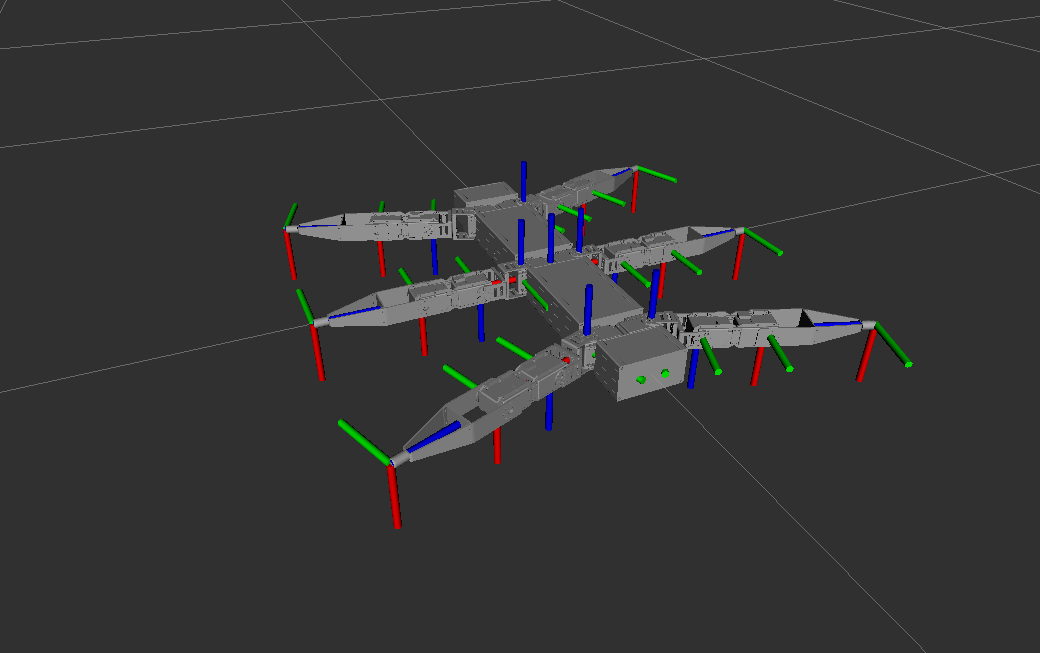
\includegraphics[height=8cm]{kapitel4/akrobat-rviz}
  \caption{Darstellung des Akrobats im rviz}
  \label{Kap4:AkrobatRviz}
\end{figure}

Für das spätere Hinzufügen des Akrobats in die \textit{Gazebo}-Simulation müssen neben der Visualisierung, die für den rviz ausreichend war, noch weitere Anpassungen am Roboter-Modell vorgenommen werden:
\begin{itemize}
  \item Aufsetzen des Kollisionsmodells durch das Attribut <collission>
  \item Aufsetzen der Massenträgheit durch das Attribut <inertia>
\end{itemize}

\subsubsection{Aufsetzen des Kollisionsmodells}

Das Kollisionsmodell muss für jedes Körperteil einzeln definiert werden. Es wird durch ein Ursprung und einem geometrischen Objekt definiert. Das \ac{ROS} stellt hierfür eine Schnittstelle zur Verfügung, die zwei Möglichkeiten anbietet. Zum einen können einfache geometrische Objekte wie ein Zylinder oder ein Quader als Kollisionsmodell definiert werden. Dies ist in unserem Fall nicht möglich, da sich die Beinsegmente nicht exakt durch einzelne geometrische Objekte modellieren lassen. Daher ist es sinnvoll auf die zweite Variante zurückzugreifen und die exakten 3D-Modelle über die stl-Dateien als Kollisionsmodelle anzugeben. Da diese viel detaillierter sind, wird daher zwar mehr Rechenleistung benötigt, aber auch die physikalischen Bewegungen sehen realer aus. Eine Möglichkeit wäre es die 3D-Modelle mittels MeshLab \autocite{LocalChapterEvents:ItalChap:ItalianChapConf2008:129-136} runterzurechnen, so dass sie später besser von Gazebo verarbeitet werden können, da sie optimiert sind.

\subsubsection{Aufsetzen der Massenträgheit}

\begin{figure}[b!]
  \centering
  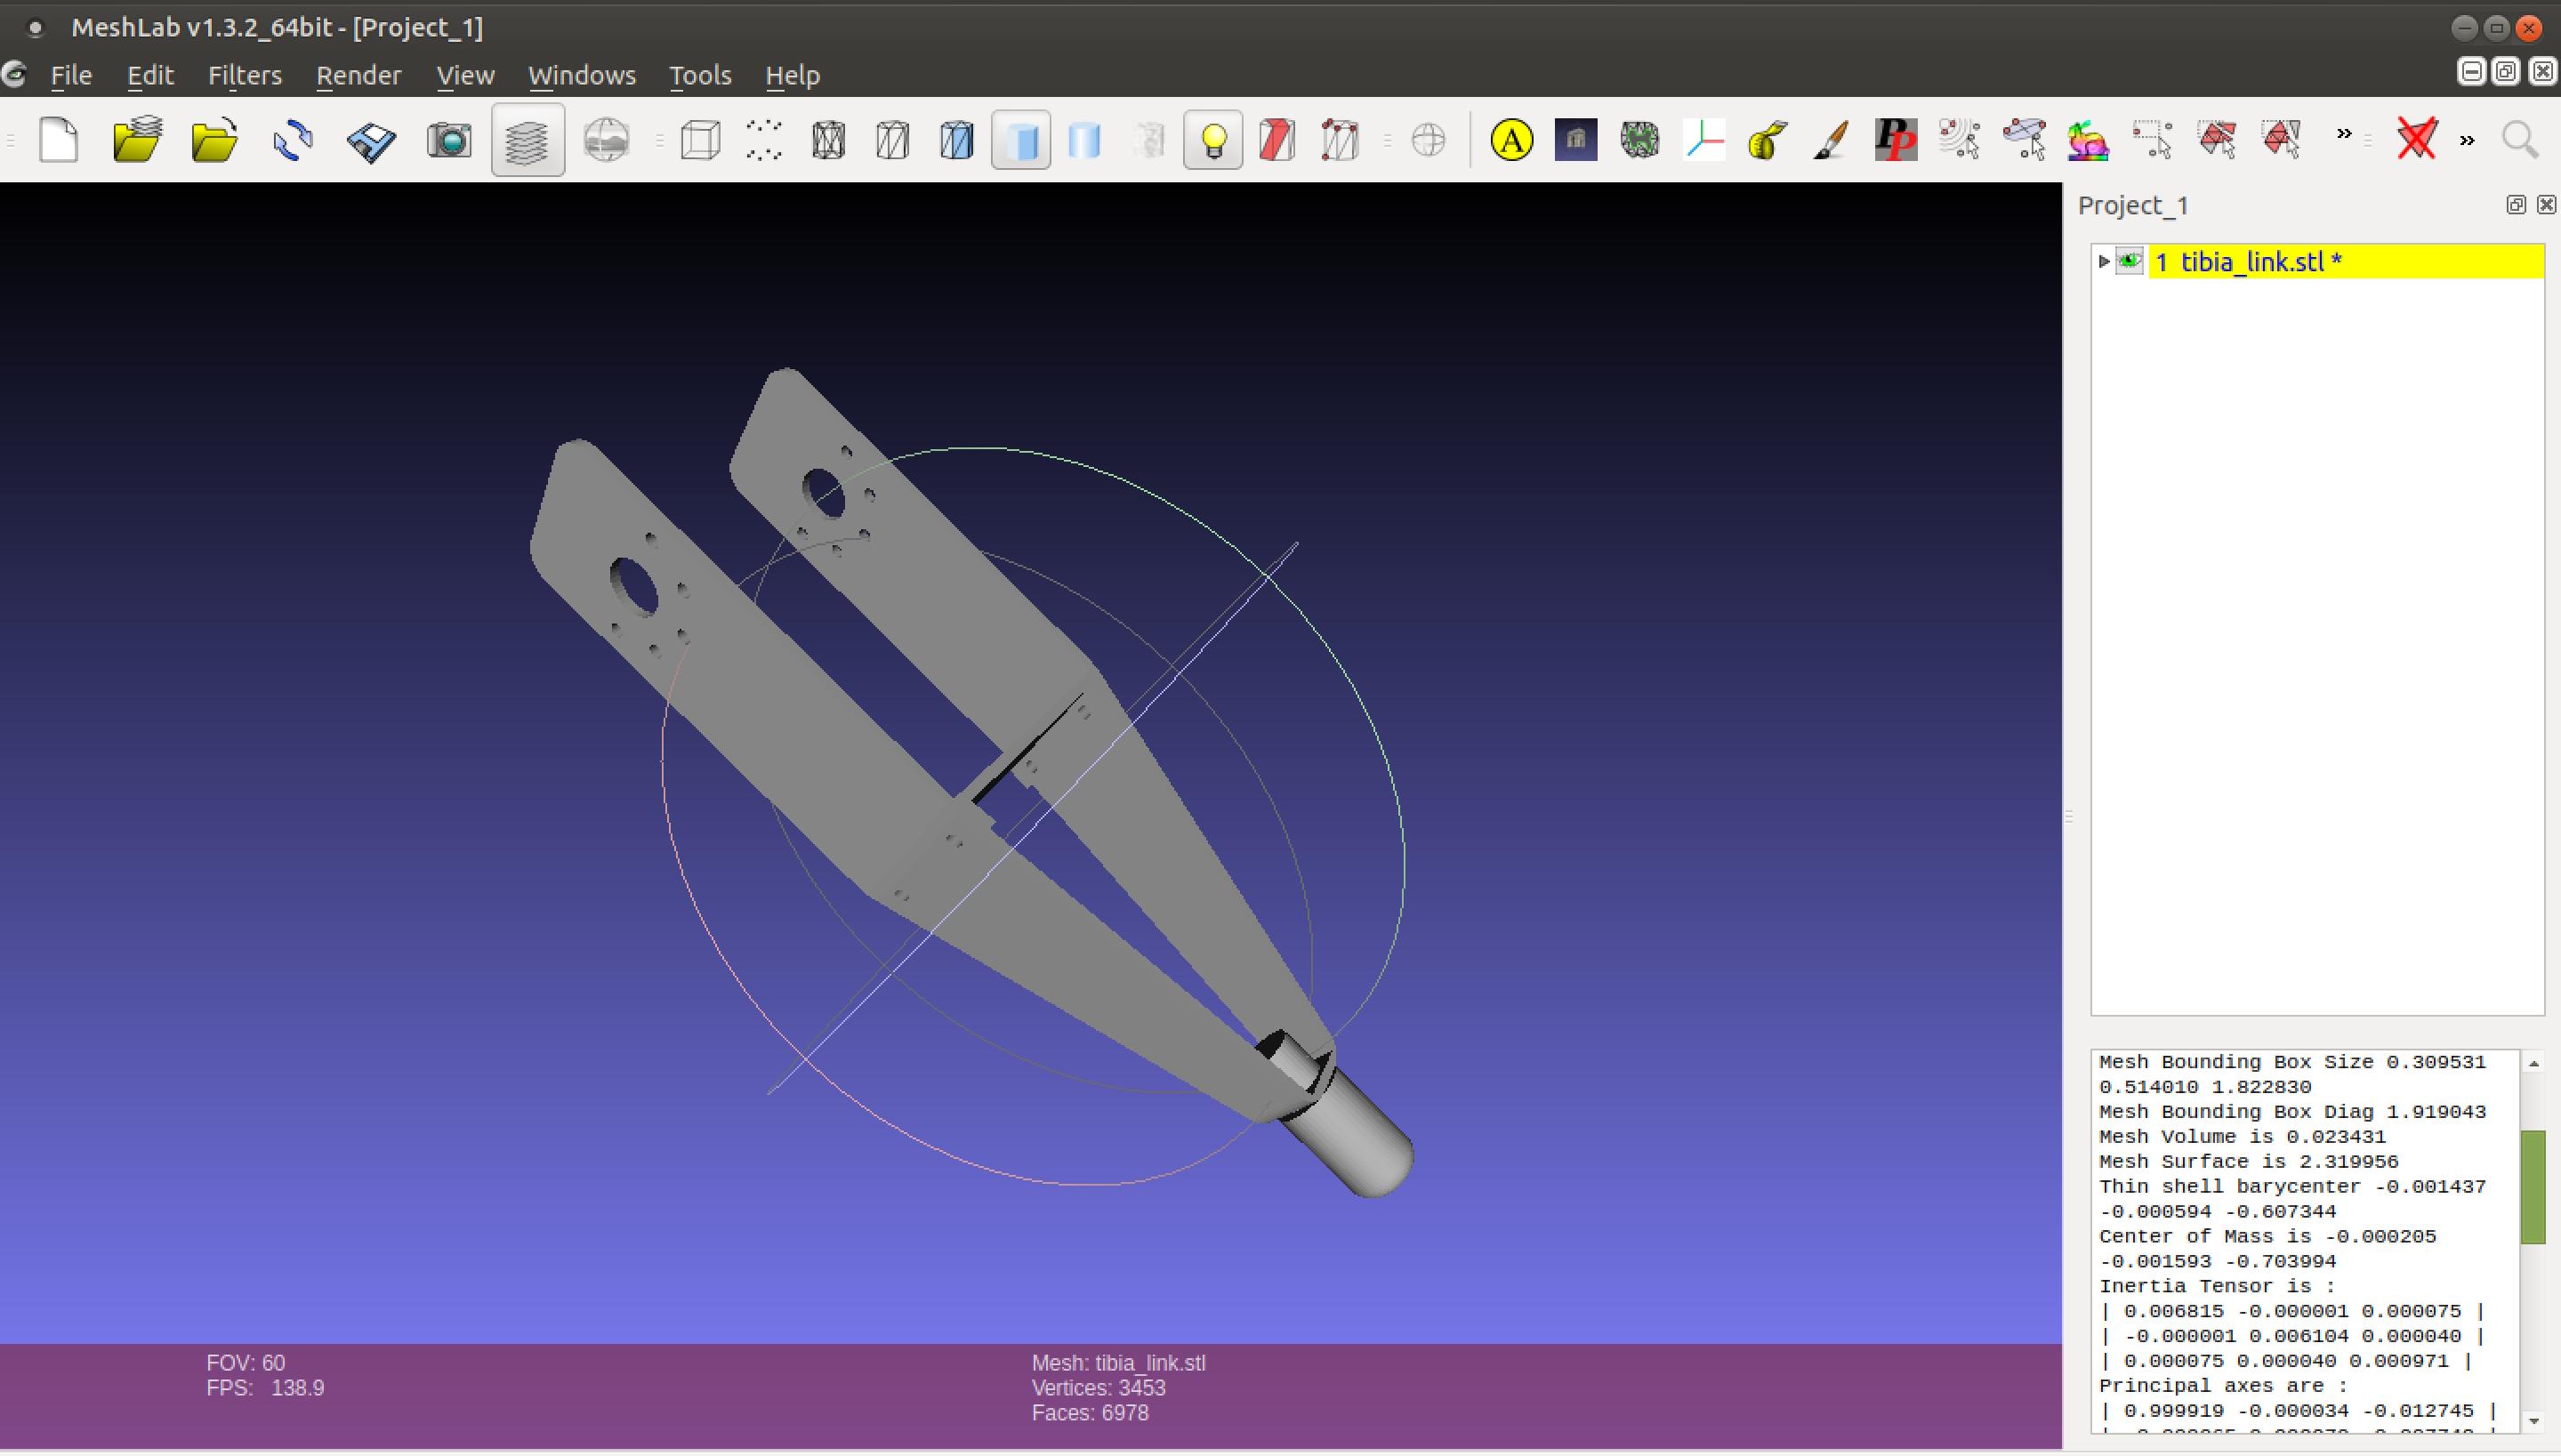
\includegraphics[height=8cm]{kapitel4/meshlab-inertia}
  \caption{Auslesen der Trägheitsmomente mit MeshLab}
  \label{Kap4:MeshLabInertia}
\end{figure}

Ebenfalls muss die Massenträgheit für jedes Körperteil einzeln definiert werden. Dabei wird eine Masse sowie das Trägheitsmoment angegeben. Die Masse lässt sich durch Wiegen der einzelnen Körperteile herausfinden. Um das Trägheitsmoment für das jeweilige Körperteil herauszufinden, bietet Gazebo die Möglichkeit die Werte über MeshLab auszulesen und umzuwandeln \autocite{gazebo-inertial}. \autoref{Kap4:MeshLabInertia} zeigt die Extraktion der Trägheitsmomente aus MeshLab. Dies erfolgt über mehrere Schritte, um möglichst genaue Ergebnisse zu erhalten:
\begin{itemize}
  \item Skalierung in MeshLab mit Faktor 10 bis 100
  \item Automatische Berechnung der Trägheitsmomente in MeshLab
  \item Teilen des Ergebnisses durch den zuvor skalierten Faktor
  \item Multiplizieren des Ergebnisses mit der berechneten Masse
  \item Teilen des Ergebnisses durch das berechnete Volumen
  \item Eintragen der berechneten Werte in \ac{ROS}
\end{itemize}

\subsection{Definition der Gelenkmotoren mittels ros\_control}

Das zuvor aufgesetzte Robotermodell könnte nun in Gazebo angezeigt werden. Allerdings ist dieses noch nicht durch Eingaben von außen beweglich, da keine Gelenkmotoren definiert sind. Diese werden in diesem Abschnitt behandelt.

Hierbei hat sich das Paket \textit{ros\_control} als geeignet herausgestellt. Für das Aufsetzen des Pakets wird eine Konfigurationsdatei für die Definition aller Controller benötigt. Außerdem muss im Robotermodell ein Gelenk auf einen Controller abgebildet werden, damit das Gelenk angesteuert werden kann. Außerdem müssen zwei wesentliche Plugins eingebunden und konfiguriert werden:
\begin{itemize}
  \item gazebo\_ros\_control
  \item p3d\_base\_controller
\end{itemize}

Abschließend muss die Konfigurationsdatei geladen und zwei \ac{ROS}-Nodes gestartet werden. Dies ist zum einen der \textit{robot\_state\_publisher}, der die publizierten Bewegungen an den Roboter weitergibt, sowie ein \textit{controller\_manager}, der letztendlich die einzelnen Gelenke in der Simulation bewegt. Hier lässt sich statt dem \textit{controller\_manager} auch direkt ein \textit{dynamixel\_manager} anbinden, so dass später leicht zwischen Simulation und dem realen Roboter gewechselt werden kann. Durch die Einbindung existieren nun zur Laufzeit einige wichtige \ac{ROS}-Topics, wie in \autoref{Kap4:RosControlTopics} zu sehen ist.

\begin{figure}[p!]
  \centering
  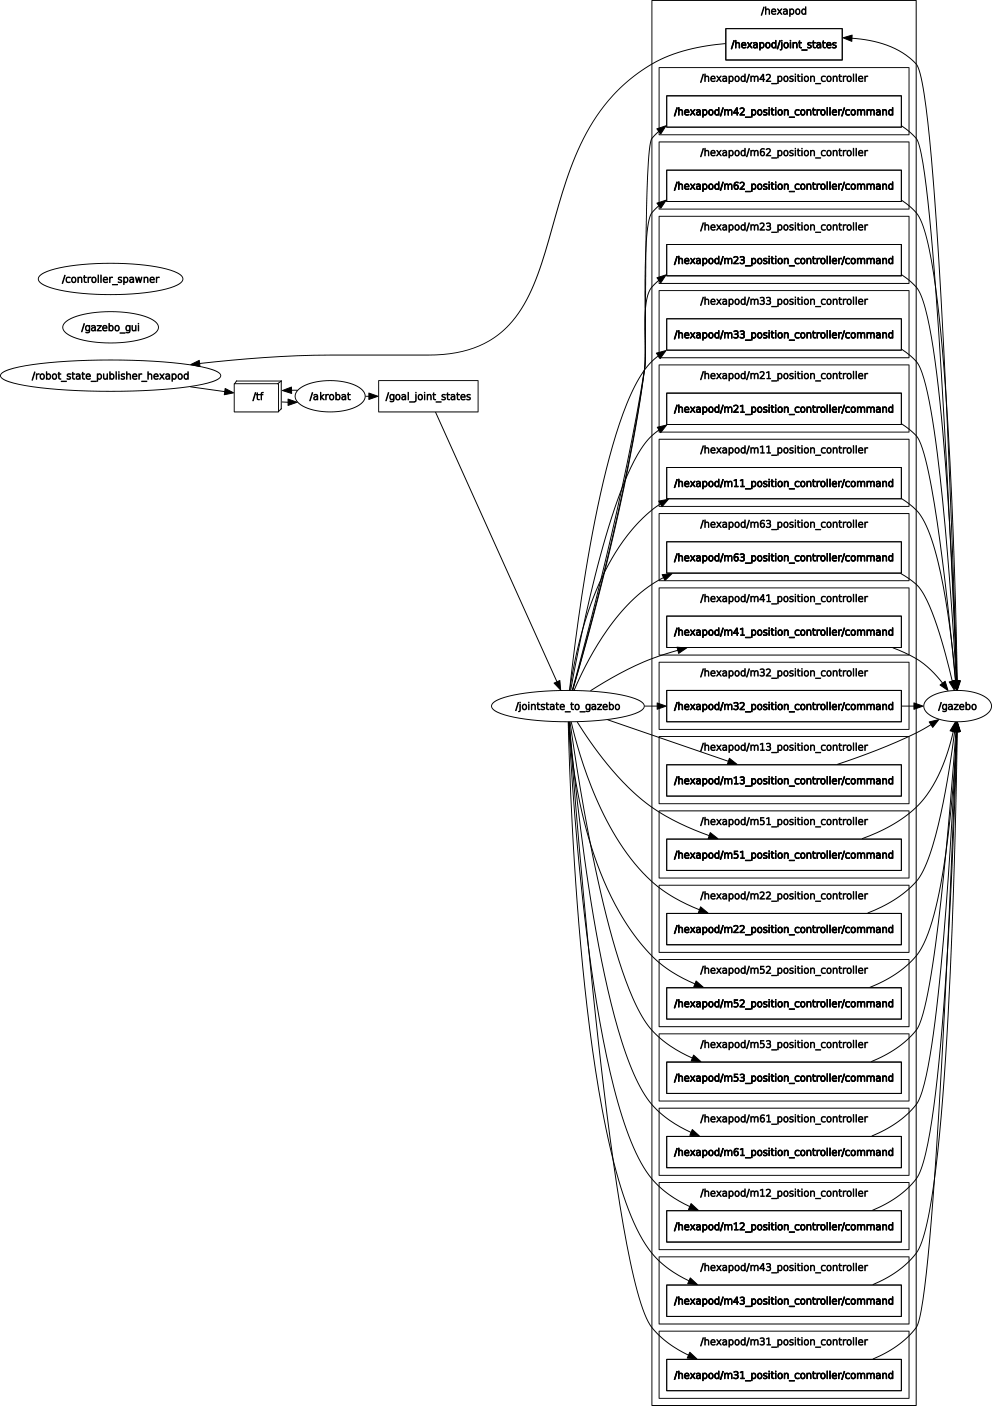
\includegraphics[height=23cm]{kapitel4/rosgraph}
  \caption{Topics für ros\_control}
  \label{Kap4:RosControlTopics}
\end{figure}

\subsection{Aufsetzen der Umgebung mittels Gazebo}

Nun fehlt nur noch die Gazebo-Umgebung. Diese lässt sich mit einem von Gazebo bereitgestellten Launch-File starten. Es besteht die Möglichkeit Parameter mitzugeben. Die folgende Auflistung beschreibt einige wichtige Parameter:
\begin{itemize}
  \item \textit{world\_name}: Dateipfad zur gewünschten Welt
  \item \textit{debug}: Gibt Informationen zur Analyse während der Laufzeit aus
  \item \textit{gui}: Startet die grafische Oberfläche
  \item \textit{paused}: Pausiert die Simulation
\end{itemize}

Damit ist das Aufsetzen des Roboters sowie der Simulationsumgebung vollständig. Der Roboter wird nun in Gazebo angezeigt, wie in \autoref{kap4:gazeboflach} zu sehen ist.

\section{Aufsetzen der Ausgangsposition}

Der Roboter wird nun zwar im Gazebo angezeigt, allerdings liegt dieser nun flach auf dem Boden. Das Ziel ist es daher, die Fußsteuerung aufzusetzen, so dass der Roboter sich zu Beginn in seine Ausgangsstellung begibt. Von dort aus wartet der Roboter auf weitere Befehle für die Bewegung.

\begin{figure}[b!]
  \centering
  \begin{subfigure}[b]{.4\linewidth}
    \centering
    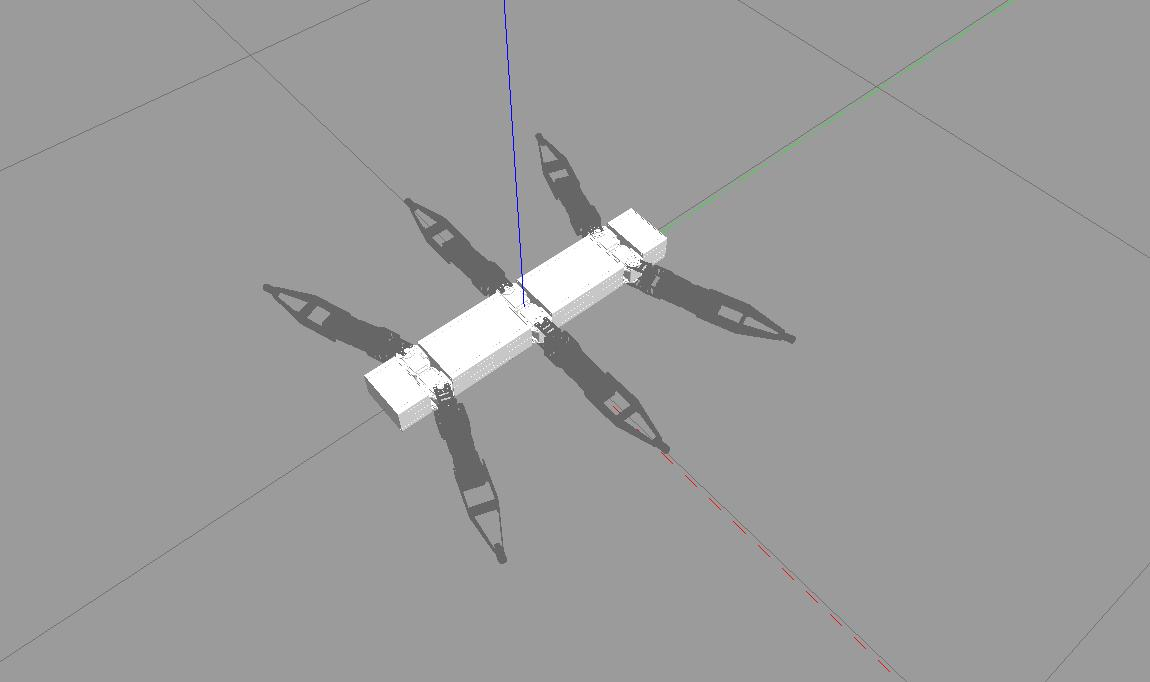
\includegraphics[width=6cm]{kapitel4/akrobat-flach}
    \subcaption{Vor Aufsetzen der Ausgangsposition}\label{kap4:gazeboflach}
  \end{subfigure}%
  \qquad
  \begin{subfigure}[b]{.4\linewidth}
    \centering
    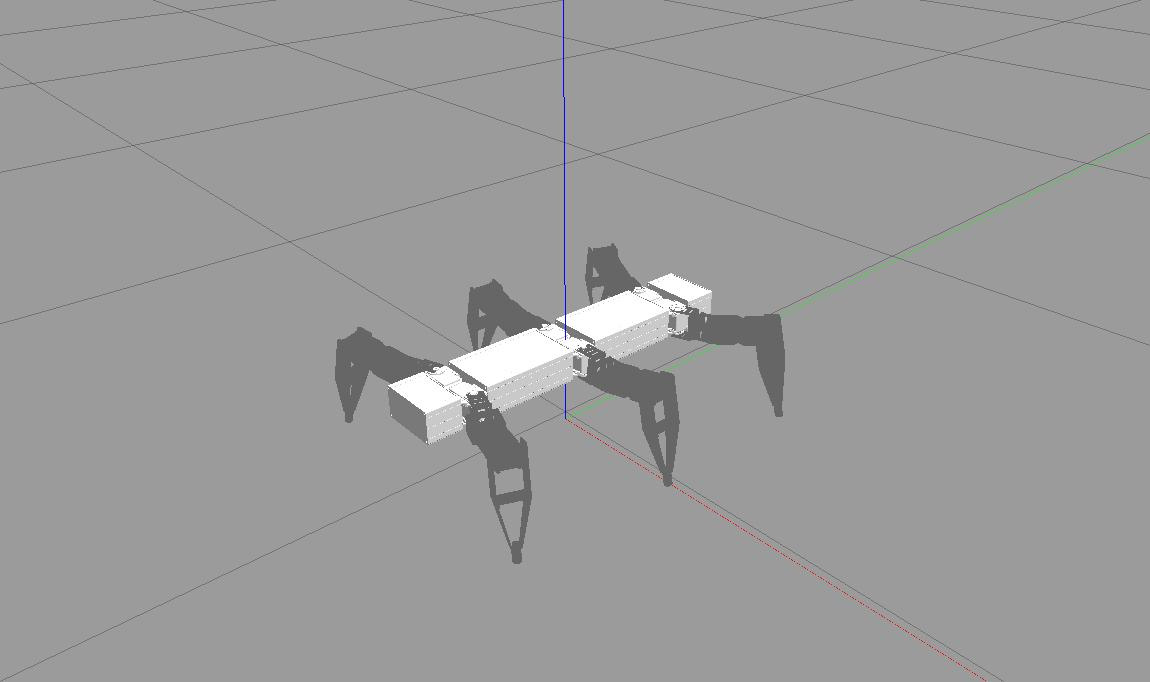
\includegraphics[width=6cm]{kapitel4/akrobat-oben}
    \subcaption{Nach Aufsetzen der Ausgangsposition}\label{kap4:gazebooben}
  \end{subfigure}\\
  \caption{Aufstehen des Akrobat in Gazebo}
  \label{kap4gazebo}
\end{figure}

Da \ac{ROS}-Nodes allgemein in einer Schleife laufen, wird der folgende Ablauf kontinuierlich ausgeführt. Der Ablauf sorgt wie in \autoref{kap4:gazebooben} zu sehen, dafür, dass der Roboter in den nächsten Durchläufen in der Ausgangsposition steht. Dies erfolgt in mehreren Schritten: 
\begin{enumerate}
  \item Zunächst wird über das \textit{TF-Framework} mit Hilfe von Transformationen und Rotationen die Ausgangsposition vom obersten Gelenk zum Endeffektor berechnet. Dies wird im weiteren Verlauf als Ausgangsposition definiert und eingelesene Bewegungen sind relativ zu dieser Position.
  \item Die dazugehörigen Winkel, die benötigt werden, um in die Ausgangsposition zu kommen, werden nun mittels \textit{inverser Kinematik} berechnet.
  \item Die drei Winkel werden nun in das Topic \textit{goal\_joint\_states} geschrieben, was ein tatsächliches Verändern der Winkel in der Simulation oder am echten Roboter verursacht. Dabei wird vorher geprüft, ob die Winkel gültig sind, d.h. dass sie sich über dem minimal und unter dem maximal erlaubten Winkel befinden. Ist das nicht der Fall, wird eine Warnung ausgegeben.
\end{enumerate}

\section{Generierung von Bewegungen als xml-Datei}

\section{Einlesen und Abspielen der Bewegungen}

\autocite{pugixml}

\section{Testen der Fußsteuerung}

- mit Hilfe von Tripod Gait
- Setup Tripod Gait
- 4 Screenshots wo man ein paar Bewegungen sieht

\section{Aufsetzen von Random Sampling}